
\documentclass{book}
\usepackage{amsmath, amsthm, graphicx, amsfonts, float}
\usepackage[english]{babel}
\graphicspath{ {./images/} }

\usepackage{geometry}
 \geometry{
 a4paper,
 total={170mm,237mm},
 left=20mm,
 top=30mm,
 }
 \usepackage[hidelinks]{hyperref}

\newcommand\at[2]{\left.#1\right|_{#2}}
\DeclareMathOperator{\sgn}{sgn}
\newcommand{\notimplies}{%
  \mathrel{{\ooalign{\hidewidth$\not\phantom{=}$\hidewidth\cr$\implies$}}}}


\title{Industrial Robotics M}
\author{Dante Piotto}
\date{spring semester 2023}


\begin{document}
\chapter{Intro to physical modelling}
\subsubsection{Engineering multiports}
Engineering multiports are Places at which subsystems can be interconnected are where power can flow between the sbusystems, and such places are called ports. Physical subsystems with one or more ports are called multiports. The variables listed for the previous multiports are called power variables, because the product of the two variables considered as functions of time is the instantaneous power flowing between the two multiports. All power variables are called either \emph{effort} ($e$) or \emph{flow} ($f$).

The power flowing through a port can be expressed as the product of an effort and a flow variable: 
\[
    P(t) = e(t)f(t)
\]
Two other types of variables (\emph{energy variables}) turn out to be important in describing dynamic systems: 
\begin{itemize}
    \item Momentum $p(t) = p_0 + \displaystyle\int_{t_0}^{t}e(\tau)d\tau$ 
    \item Displacement: $q(t) = q_0 + \displaystyle\int_{t_0}^{t}f(\tau)d\tau$ 
\end{itemize}
The \emph{energy flow} is the time integral of the power flow: 
\begin{gather*}
    E(t) = \displaystyle\int_{}^{t}P(\tau)d\tau = \displaystyle\int_{}^{t}e(\tau)f(\tau)d\tau \\
    E(t) = \displaystyle\int_{}^{t}e(\tau)dq(\tau) = \displaystyle\int_{}^{t}f(\tau)dp(\tau)
\end{gather*}
There are cases where an effort is a function of a displacement, or a flow is a function of a momentum, which implies that 
\[
    E(q) = \displaystyle\int_{}^{q}e(\bar{q})d\bar{q} \qquad E(p) = \displaystyle\int_{}^{p}f(\bar{p})d\bar{p}
\]
Multiport elements can be connected to other multiport to form systems, and power can flow through the connected ports. 

\section{Bond Graphs}
When two multiports are coupled so that the effort and flow variables become identical, the two multiports are said to have a common bond, in analogy to the bonds between component parts of molecules.

A bond graph consists of subsystems linked together by power bonds. When major subsystems are represented by words, the graph is called a word bond graph. The word bond graph serves to make som initial decisions about the representation of dynamic systems.

\subsubsection{The causal stroke}
In performing experiments, the notions of input and output arise. One must make a decision about what  is to be done at the ports. At each port, both an effort and a flow variable exist, and one can control either one but not both of these variables simultaneously. In bond graphs, the way in which inputs and outputs are specified is by means of the causal stroke: \begin{itemize}
    \item the causal stroke is a short, perpendicular line made at the end of a bond
    \item it indicates the direction in which the effort signal is directed 
    \item the end of a bond that does not have a causal stroke is the end toward which the flow's signal arrow points.
\end{itemize}

\subsubsection{Pure signal flow}
In the case of pure signal flow (transfer of information with negligible power flow), either an effort or a flow may be suppressed at many interconnection points. In this case, the bond degenerates to a single signal (active bond). In many cases, systems are designed so that only one of the power variables is important, i.e. a single signal is transmitted between two subsystems 
\begin{itemize}
    \item Electronic amplifier
    \item Ideal Ampere meter 
    \item Control system (ideal actuator)
\end{itemize}
Control systems are useed to modify the dynamic behavour of engineering systems. They require: 
\begin{itemize}
    \item Sensors
    \item Signal processors 
    \item Actuators 
\end{itemize}
It is advantageous to use composite representations in which the physical systems is represented using bond graphs and the controller is represented as a signal processor.


\chapter{Basic component models}

\section{Basic 1 port elements}
\subsubsection{1-port resistor}
an element in which the effort and flow variables at the single port are related by a static function.
\[
    e = \Phi_R(f)
\]
Where $\Phi_R(\cdot)$ is called \emph{constitutive equation}.
Usually, resistors dissipate energy, i.e. power flows into the resistor but never comes out of it. 
Pwer flows nito the port when the product of $e$ and $f$ is positive according to the sign convention shown, so power is always dissipated if the constitutive relation lies in the first and third quadrants of the $e-f$ plane.
When a resistive element is assumed to be linear, it is conventional to indicate this on the bond graph by appending a colon (:) next to R. For passive resistors, estabilsh the power sign convention by means of a half-arrow pointing towards the resistor.
\begin{center}
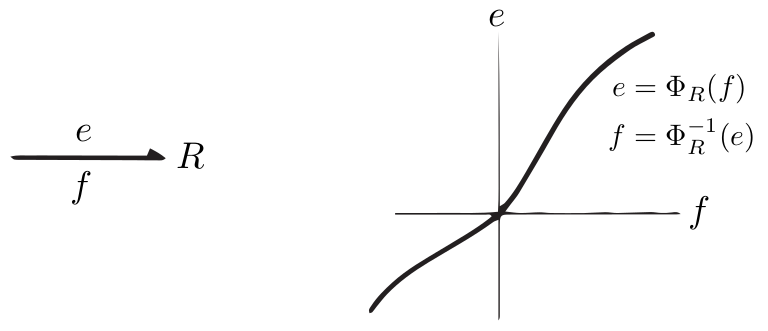
\includegraphics[width=0.45\textwidth]{1portR1}
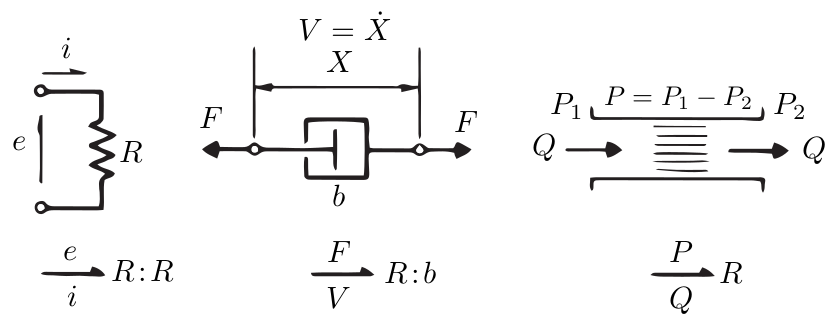
\includegraphics[width=0.45\textwidth]{1portR2}
\end{center}

\subsubsection{1-port capacitor - compliance}
1-port device in which a static constitutive relation between an effort and a displacement. 
\begin{itemize}
    \item such a device stores and gives up energy without loss 
    \item In bond graph terminology, an element that relates $e$ to $q$ is called is called a \emph{1-port capacitor} or \emph{compliance}
    \item In physical terms, a capacitor is an idealisation of devices as springs, torsion bars, electrical capacitors, gravity tanks, and hydraulic accumulators 
    \item There are idealised linear compliance elements as well as nonlinear ones
\end{itemize}
% TODO insert images slides 5-6
With the same sign convention of the resistor, we have that
\[
    E(t) = \displaystyle\int_{0}^{t}e(\tau)f(\tau)d\tau+E_0
\]
considering a change of variables $f d t = d q$ and $e=e(q)$ we get 
\[
    E(q) = \displaystyle\int_{q_0}^{q}e(\bar{q})d \bar{q} + E_0
\]
The conservation of energy for $C$ is obvious
\begin{itemize}
    \item The power flow into the port reverses and power flows out of the port 
    \item During the process, no energy is lost, i.e. it is conserved
\end{itemize}

\subsubsection{1-port inertia}
Energy storing 1-port where the momentum $p$ is related to the flow $f$ by a static constitutive law. It is the dual of the capacitor. 
\begin{itemize}
    \item it is used to model inductance effects in electrical systems, and mass or inertia effects in mechanical or fluid systems.
\end{itemize}
As before we have 
\[
    E(t) = \displaystyle\int_{0}^{t}e(\tau)f(\tau)d\tau+E_0 
\]
by considering a change of variables $edt=dp$ and $f=f(p)$
\[
    E(p) = \displaystyle\int_{p_0}^{p}f(\bar{p})d\bar{p}+E_0
\]
\subsubsection{effort source and flow source}
\begin{itemize}
    \item an effort or flow is maintained reasonably constant, or constrained to be some particular function of time 
    \item a source maintains one of the power variables constant or a specified function of time no matter how large the other variable may be
\end{itemize}
It is possible to incorporate a modulation in the source element, thus obtaining a MSE of a MSF. Many physical devices function as amplifiers or transducers but are inadequately modelled as simple controlled sources.

\section{Basic 2-port elements}

The 2-ports to be discussed here are ideal in the sense that power is conserved ($e_1(t)f_1(t) = e_2(t)f_2(t)$). Let us consider a conservative 2-port with a through power sign convention
% TODO insert image slide 13 
\begin{itemize}
    \item Transformer ($TF$): $e_1 = me_2, \quad mf_1=f_2$
    \item Gyrator ($GY$): $e_1=rf_2, \quad rf_1=e_2$
\end{itemize}

The scalign ration for a $TF$ or a $GY$ can be time-dependent. In mechanics, the MTF is particularly important and may be used to represent geometric transformations or kinematic linkages.

\section{3-port junction elements}
3-port power conserving elements that serve to interconnect other multiports into subsystems or system models 
\begin{itemize}
    \item They are the most fundamental ideas behind bond graph formalism
    \item they are an abstraction of the parallel and series connections of electrical circuits 
    \item they appear in all physical domains
\end{itemize}
\subsubsection{0-junction}
\[
    e_1(t)=e_2(t)=e_3(t)\\
    f_1(t)+f_2(t)+f_3(t)=0
\]
\subsubsection{1-junction}
\[
    f_1(t)=f_2(t)=f_3(t)\\
    e_1(t)+e_2(t)+e_3(t)=0
\]
% TODO images slide 18

\section{Causality}
\subsubsection{basic 1-ports}
\begin{itemize}
    \item The 1-port resistor is normally indifferent to the causality imposed upon it, so there are two possibilities: 
        \[
            e = \Phi_R(f) \qquad f = \Phi_R^{-1}(e)
        \]
    \item The constitutive law of 1-port capacitor is a static relation between effort and displacement, which means that 
        \[
            e = \Phi_C^{-1}(\int_{}^{t}fd\tau) \qquad f = \displaystyle\frac{d}{dt}\Phi_C(e)
        \]
    \item Dually, the constitutive law of 1-port inertia is a static relation between flow and momentum
        \[
            f = \Phi_I^{-1}(\int_{}^{t}ed\tau) \qquad e = \displaystyle\frac{d}{dt}\Phi_I(f)
        \]
        For both, the integral causality form is preferred to the differential causality.
\end{itemize}
\subsubsection{basic 2- and 3-ports}
For basic 2-ports, there are two possible causal assignments. As soon as $e$ or $f$ is assigned as an input, the other one is constrained by the constitutive relation. Similar cnosiderations are valid also for 3-ports.

\chapter{System Models in Different Domains}
\section{Electrical Systems}
Any electrical circuit can be modelled by a bond graph containing elements of the set $\{0,1,R,C,I,S_e,S_f\}$. The elements $TF$ and $GY$ are not included. 
\subsection{Circuit construction procedure}
\begin{itemize}
    \item Assign a power conventin to the circuit schematic diagram: this is done by showing the positive voltage drop and current directions.
    \item Label each node voltage on the circuit schematic diagram and use a 0-junction to represent each node voltage 
    \item Establish the positive voltage drops across the circuit elements using 1-junctions: by properly directing the half-arrows on 1-junctions, the voltage drop can be established across each bond graph element
    \item Choose a ground and remove all bonds that have zero power
    \item Simplify the bond graph by using "bond graph identities"
\end{itemize}
An electrical network is an extension of electrical circuits to include idealised transformers and gyrators.
\begin{itemize}
    \item an electrical transformer is a common electromagnetic device used to step voltages up or down while doing the opposite to the current 
    \item Electrical gyrators are exhibited in Hall effect transducers, where voltage across a semiconductor material is related to a current through the material perpendicular to the voltage drop direction.
\end{itemize}

\section{Mechanical systems}
\subsection{Mechanics of translation}
The construction procedure for the bond graph is dual to that for electrical systems: 
\begin{itemize}
    \item representing system velocities using 1-junctions
    \item create the appropriate relative velocities using 0-junctions
\end{itemize}



\section{Hydraulic and acoustic circuits}





\chapter{Causality and system equations}
Hamiltonian equations are coupled first order differential equations. 






































\end{document}
